%%%%%%%%%%%%%%%%%%%%%%%%%%%%%%%%%%%%%%%%%%%%%%%%%%%%%%%%%%%%
% Theory book for guitarists
%
%%%%%%%%%%%%%%%%%%%%%%%%%%%%%%%%%%%%%%%%%%%%%%%%%%%%%%%%%%%%

%----------------------------------------------------------------------------------------
%	PACKAGES AND DOCUMENT CONFIGURATIONS
%----------------------------------------------------------------------------------------

\documentclass{article}

\usepackage{parskip}
\usepackage[shortlabels]{enumitem}
%\usepackage[version=3]{mhchem} % Package for chemical equation typesetting
%\usepackage{siunitx} % Provides the \SI{}{} and \si{} command for typesetting SI units
\usepackage{graphicx} % Required for the inclusion of images
%\usepackage{natbib} % Required to change bibliography style to APA
\usepackage{amsmath,amssymb} % Required for some math elements 
\usepackage{caption}
\usepackage{subcaption}
\usepackage{hyperref}
\setlength\parindent{0pt} % Removes all indentation from paragraphs
\usepackage{booktabs}
\usepackage{pgfplots}

\usepackage{changepage}
\usepackage{multirow}


\renewcommand{\labelenumi}{\alph{enumi}.} % Make numbering in the enumerate environment by letter rather than number (e.g. section 6)

%% Recherche des images dans les répertoires.
\graphicspath{{./figures/}{./dia/}{./gnuplot/}}

\title{ Music theory for guitar nerds  } % Title
\author{ Jean-Hughes \textsc{Fournier L.} } % Author name
\date{\today} % Date for the report

% Plan:
%
% 1. Intervals (Why intervals are consonant or dissonant?, Harmonic series, harmonic entropy, battement)
%      1.1 Harmonic series
%      1.2 Consonance and dissonance
% 2. Scales    (Major scale, minor scales, pattern on fretboard)
% 3. Chords    (Triad, tetrad, pentad)
%  3.1 Chord progressions (Circle of fifths)
% 4. Modes     (Table of modes)
% 5. Arpeggios



%***********************************************************************************************************************************************
\begin{document}

\maketitle % Insert the title, author and date
\newpage
\tableofcontents
\newpage

\begin{itemize}
	\item Gives the recipe not just examples
	\item If you give a man a fish, you feed him for a day. If you teach a man to fish, you feed him for a lifetime
\end{itemize}

%%%%%%%%%%%%%%%%%%%%%%%%%%%%%%%%%%%%%%%%%%%%%%%%%%%%%%%%%%%%%%%%%%%%%%%
\section{Intervals: where do notes come from?}

%Names of the interval comes from the diatonic scale. In C major scale (C-D-E-F-G-A-B-C) that scale G$\#$ is the augmented 5. In C minor scale (C-D-Eb-F-G-Ab-Bb) G$\#$ is the minor sixth.

\subsection{Harmonic series}

% Figure 
\begin{figure}[h!]
	\centering
	\hspace*{0cm}
	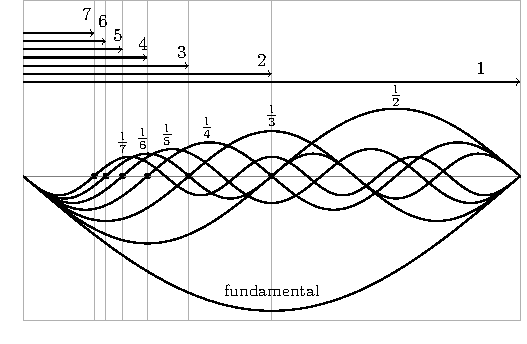
\includegraphics[scale=1.0, trim= {0cm 0cm 0cm 0cm}, clip]{serie_harmonique/main.pdf}
	\caption{The harmonic series}
	\label{fig}
\end{figure} 

%% Table

% Table
\begin{table*}[!h]
	\caption{Intervals and }
	\centering
	\begin{tabular}{|c|c|c|c|c|c|c|c|}
		\hline 
		\multicolumn{5}{|c|}{\textbf{Harmonics}}  &  \textbf{Ratio to fundamental} & \textbf{Intervals}  & \textbf{Equal Temperament}  \\
		\hline
		1 & 2 & 4 & 8 & 16  & 1,2,3,4 & unison/octave      & 1.000 \\
		\hline
		  &   &   &   & 17  & $17/16=1.0625$ & minor second & 1.059 \\
		  \hline
		  &   &   & 9 & 18   & $9/8=1.125$ & major second  & 1.122 \\
		  \hline
		  &   &   &   & 19    & $19/16=1.1875$ & minor third  & 1.189 \\
		  \hline
		  &   & 5 &10 & 20    & $5/4=1.2500$ & major third & 1.260 \\
		  \hline
		  &   &   &   & 21   & $21/16=1.3125$ & fourth & 1.335 \\
		  \hline
		  &   &   & 11& 22  & $11/8=1.375$ & \multirow{2}{*}{tritone}  & \multirow{2}{*}{$1.414$} \\
		  &   &   &   & 23  & $23/16=1.4375$ &   &  \\
		  \hline
		  & 3 & 6 &12 & 24 & $3/2=1.500$ &  fifth  & 1.498 \\
		  \hline
		  &   &   &  & 25 & $25/16=1.5625$ & \multirow{2}{*}{minor sixth} &\multirow{2}{*}{$1.587$}\\
		  &   &   &13 & 26 & $13/8 = 1.625$              &             &  \\
		  \hline
		  &   &   &   & 27    & $27/16=1.6875$ & major sixth & 1.682 \\
		  \hline
		  &   & 7 & 14& 28 & $7/4=1.7500$ & \multirow{2}{*}{minor seventh} & \multirow{2}{*}{$1.782$}  \\
		  &   &   &   & 29 & $29/16 = 1.8125$         &             &  \\
		  \hline
		  &   &   & 15& 30 & $15/8=1.875$ & \multirow{2}{*}{major seventh} & \multirow{2}{*}{$1.888$} \\
		  &   &   &   & 31 & $31/16=1.9375$        &  &  \\
		\hline
	\end{tabular}
	\label{tab: }
\end{table*}




% Table
% Source: https://hellomusictheory.com/learn/intervals/
\begin{table*}[!h]
	\caption{Intervals chart in relation to C note. Minor (m or ``-''), major (M or ``maj''), augmented (A or ``aug'' or ``$\#$'' or ``$+$'') and diminished (d or ``dim'' or ``b''). }
	\centering
	\begin{adjustwidth}{-2cm}{}
	\begin{tabular}{clclcl}
		\hline 
		\textbf{Semitones} & \textbf{Name} & \textbf{Notation} & \textbf{Songs}  \\
		\hline
		0 & Perfect unison            & P1 & -   \\
		\hline
		1 & Minor second              & m2 & JAWS theme \\
		2 & Major second              & M2 & \textbf{Frè-re} Jacques  \\
		\hline
		3 & Minor third               & m3 & Iron Man by Black Sabbath\\
		4 & Major third               & M3 & "\textbf{Oh-When} the Saints" \\
		\hline
		5 & Perfect fourth            & P4 & Here Comes the Bride (Wedding song) \\
		\hline
		6 & Triton                    & T  & "\textbf{The - Simp}-sons" \\ 
		\hline
		7 & Perfect fifth             & P5 &  "\textbf{Twinkle - Twinkle} Little Star"   \\
		\hline
		8 & Minor sixth               & m6 &  The Entertainer \\
		9 & Major sixth               & M6 &  Jingle Bells ("\textbf{Dash-ing} through the snow")   \\
		\hline
		10 & Minor seventh            & m7 &  Theme song Star Trek : The Original Series\\
		11 & Major seventh            & M7 &  Take On Me ("Take-on")  \\
		\hline
		12 & Perfect octave           & P8 &  "\textbf{Some-where} over the rainbow" \\
		\hline
		13 & Minor ninth              & m9 &  - \\
		14 & Major ninth              & M9 &  - \\
		\hline
		16 & Diminished eleventh      & d11 & - \\
		17 & Perfect eleventh         & P11 & - \\
		18 & Augmented eleventh       & A11 & - \\
		\hline
		20 & Minor thirteenth         & m13 & - \\
		21 & Major thirteenth         & M13 & - \\
		\hline
	\end{tabular}
	\end{adjustwidth}
	\label{tab: }
\end{table*}


% ****************************************************************************
\subsection{Consonance and dissonance}

% Figure 
\begin{figure}[h!]
	\centering
	\hspace*{0cm}
	\includegraphics[scale=0.03, trim= {0cm 0cm 0cm 0cm}, clip]{Harmonic_entropy.png}
	\caption{Harmonic entropy}
	\label{fig}
\end{figure}

% Figure 
\begin{figure}[h!]
	\centering
	\hspace*{0cm}
	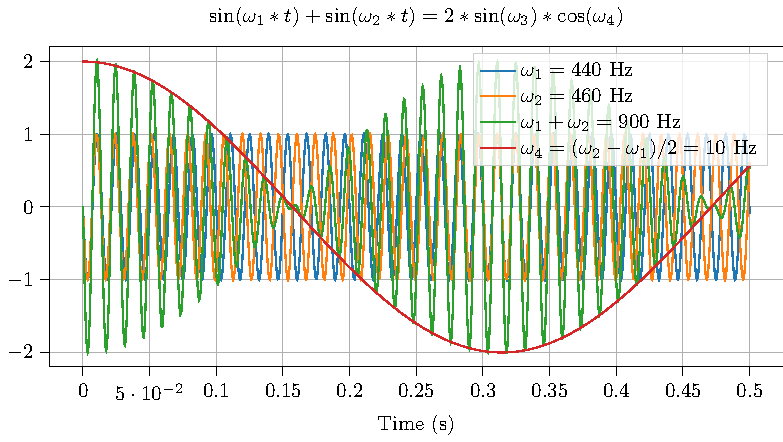
\includegraphics[scale=0.5, trim= {0cm 0cm 0cm 0cm}, clip]{battement/main.pdf}
	\caption{Beat tone}
	\label{fig}
\end{figure}


%%%%%%%%%%%%%%%%%%%%%%%%%%%%%%%%%%%%%%%%%%%%%%%%%%%%%%%%%%%%%%%%%%%%%%%
% Interval of notes create scales
\newpage
\section{Relation between scales}

Modes ranked by brightness: Super-locrian, locrian, phrygian, aeolian, dorian, mixolydian, major, lydian, lydian augmented

% Insert the table from an external file
%\input{scales_table.tex}

% Table  
\begin{table*}[!h]
	\caption{Scales formula (relative to the major scale)}
	\begin{adjustwidth}{-2.5cm}{}
	\begin{tabular}{l|ccc cccc|l}
		Scale name  & \multicolumn{7}{c}{Formula} & Comment \\ 
		\hline \hline \vspace{-0.4cm} \\
		\textcolor{yellow!90!black}{Major} & \textcolor{yellow!90!black}{1}  
										    & \textcolor{yellow!90!black}{2}  
										    & \textcolor{yellow!90!black}{3}  
										    & \textcolor{yellow!90!black}{4} 
										    & \textcolor{yellow!90!black}{5}  
										    & \textcolor{yellow!90!black}{6} 
										    & \textcolor{yellow!90!black}{7} & \\ 
		Pentatonic Major   & 1 & 2  & 3  &   -   & 5  & 6  &  - &  \\ 
		\textcolor{red!60!white}{Natural minor}      & \textcolor{red!60!white}{1} 
													  & \textcolor{red!60!white}{2} 
													  & \textcolor{red!60!white}{b3} 
													  & \textcolor{red!60!white}{4}      
													  & \textcolor{red!60!white}{5}   
													  & \textcolor{red!60!white}{b6} 
													  & \textcolor{red!60!white}{b7} 
													  & \\
		Pentatonic minor        & 1 &  - & b3 & 4  & 5  & - &  b7 &  \\ 
		Harmonic minor          & 1 & 2  & b3 & 4  & 5  & b6 & \textcolor{black}{\fbox{7}}  &  \\
		Melodic minor           & 1 & 2  & b3 & 4  & 5  & \textcolor{black}{\fbox{6}}  & 7  &  \\ 
		
		\hline
		
		\textcolor{yellow!90!black}{Ionian (Major)}  & \textcolor{yellow!90!black}{1}  
											  		  & \textcolor{yellow!90!black}{2}  
											  		  & \textcolor{yellow!90!black}{3}  
											  		  & \textcolor{yellow!90!black}{4} 
											  		  & \textcolor{yellow!90!black}{5}  
											  		  & \textcolor{yellow!90!black}{6} 
											  		  & \textcolor{yellow!90!black}{7} & \\ 
		\textcolor{green!60!white!70!black}{Dorian}  & \textcolor{green!60!white!70!black}{1} 
													  & \textcolor{green!60!white!70!black}{2} 
													  & \textcolor{green!60!white!70!black}{b3} 
													  & \textcolor{green!60!white!70!black}{4} 
													  & \textcolor{green!60!white!70!black}{5}  
													  & \textcolor{green!60!white!70!black}{6} 
													  & \textcolor{green!60!white!70!black}{b7} & Mad world, So What \\ 
		\textcolor{cyan}{Phrygian}                   & \textcolor{cyan}{1} 
													  & \textcolor{cyan}{b2} 
													  & \textcolor{cyan}{b3} 
													  & \textcolor{cyan}{4} 
													  & \textcolor{cyan}{5}  
													  & \textcolor{cyan}{b6} 
													  & \textcolor{cyan}{b7} & Symphony of destruction\\ 
		\textcolor{blue!50!white}{Lydian}            & \textcolor{blue!50!white}{1} 
													  & \textcolor{blue!50!white}{2}
													  & \textcolor{blue!50!white}{3}  
													  & \textcolor{blue!50!white}{$\#$4} 
													  & \textcolor{blue!50!white}{5}  
													  & \textcolor{blue!50!white}{6}  
													  & \textcolor{blue!50!white}{7}  
													  &  Legend of Zelda\\ 
		\textcolor{blue!50!red!50!white}{Mixolydian} & \textcolor{blue!50!red!50!white}{1} 
													  & \textcolor{blue!50!red!50!white}{2} 
													  & \textcolor{blue!50!red!50!white}{3} 
													  & \textcolor{blue!50!red!50!white}{4}    
													  & \textcolor{blue!50!red!50!white}{5}
													  & \textcolor{blue!50!red!50!white}{6}
													  & \textcolor{blue!50!red!50!white}{b7}
													  & Clock by Coldplay\\ 
		\textcolor{red!60!white}{Aeolian (natural minor)} & \textcolor{red!60!white}{1} 
													  & \textcolor{red!60!white}{2} 
													  & \textcolor{red!60!white}{b3} 
													  & \textcolor{red!60!white}{4}      
													  & \textcolor{red!60!white}{5}   
													  & \textcolor{red!60!white}{b6} 
													  & \textcolor{red!60!white}{b7} 
													  & Smell Like Teen Spirit\\
		\textcolor{orange!80!white}{Locrian}         & \textcolor{orange!80!white}{1}
													  & \textcolor{orange!80!white}{b2} 
													  & \textcolor{orange!80!white}{b3}
													  & \textcolor{orange!80!white}{4}   
													  & \textcolor{orange!80!white}{b5}
													  & \textcolor{orange!80!white}{b6}
													  & \textcolor{orange!80!white}{b7}
													  & Rush-YYZ intro\\ 
		
		\hline 
		\textcolor{yellow!90!black}{Ionian b6}    & \textcolor{yellow!90!black}{1} 
												   & \textcolor{yellow!90!black}{2}
												   & \textcolor{yellow!90!black}{3}
												   & \textcolor{yellow!90!black}{4}
												   & \textcolor{yellow!90!black}{5}
												   & \textcolor{yellow!90!black}{\textcolor{yellow!90!black}{\fbox{b6}}} 
												   & \textcolor{yellow!90!black}{7}\\ 
		\textcolor{green!60!white!70!black}{Dorian {\footnotesize $\#$}4} (4$^{\textrm{th}}$ Harm. min) & \textcolor{green!60!white!70!black}{1} 
																							& \textcolor{green!60!white!70!black}{2}  
																							& \textcolor{green!60!white!70!black}{b3} 
																							& \textcolor{green!60!white!70!black}{\fbox{\textcolor{green!60!white!70!black}{{\footnotesize $\#$}4}}} 
																							& \textcolor{green!60!white!70!black}{5}  
																							& \textcolor{green!60!white!70!black}{6}  
																							& \textcolor{green!60!white!70!black}{b7} 
																						    & \\
		\textcolor{cyan}{Phrygian dominant} (5th Harm. min) & \textcolor{cyan}{1} 
													  & \textcolor{cyan}{b2} 
													  & \textcolor{cyan}{\fbox{\textcolor{cyan}{3}}}
													  & \textcolor{cyan}{4} 
													  & \textcolor{cyan}{5}  
													  & \textcolor{cyan}{b6} 
													  & \textcolor{cyan}{b7} & Flamenco, egyptian \\
		\textcolor{blue!50!white}{Lydian dominant} (4th Melo. min)  & \textcolor{blue!50!white}{1} 
																	  & \textcolor{blue!50!white}{2}
																	  & \textcolor{blue!50!white}{3} 
																	  & \textcolor{blue!50!white}{{\footnotesize $\#$}4 }
																	  & \textcolor{blue!50!white}{5}
																	  & \textcolor{blue!50!white}{6} 
																	  & \textcolor{blue!50!white}{\textcolor{blue!50!white}{\fbox{b7}}} 
																	  & Prog futuristic, Simpsons theme\\  
		\textcolor{blue!50!red!50!white}{Mixolydian b6} (5th Melo. min)  & \textcolor{blue!50!red!50!white}{1} 
																		   & \textcolor{blue!50!red!50!white}{2}  
																		   & \textcolor{blue!50!red!50!white}{\textcolor{blue!50!red!50!white}{\fbox{3}} } 
																		   & \textcolor{blue!50!red!50!white}{4}
																		   & \textcolor{blue!50!red!50!white}{5} 
																		   & \textcolor{blue!50!red!50!white}{b6}  
																		   & \textcolor{blue!50!red!50!white}{b7} 
																		   & Prog rock \\
		(or Aeolian dominant) & & & &   & & & &\\
		Neapolitan minor                   & \textcolor{black}{1} 
													  & \textcolor{black}{b2} 
													  & \textcolor{black}{b3} 
													  & \textcolor{black}{4} 
													  & \textcolor{black}{5}  
													  & \textcolor{black}{b6} 
													  & \textcolor{black}{7} &\\                                                                                
		\hline 
		Bizantine scale (double harmonic major)      & \textcolor{black}{1} 
													  & \textcolor{black}{b2} 
													  & \textcolor{black}{3} 
													  & \textcolor{black}{4} 
													  & \textcolor{black}{5}  
													  & \textcolor{black}{b6} 
													  & \textcolor{black}{7} & Opeth - Bleak\\
	    Lydian $\#$2,$\#$6                           & & & & & & & \\
	    Ultra-Phrygian                               &1 &b2 &b3 &b4 &5 &b6 &bb7 \\
		Hungarian minor (double harmonic minor)      & \textcolor{black}{1} 
													  & \textcolor{black}{2} 
													  & \textcolor{black}{b3} 
													  & \textcolor{black}{$\#$4} 
													  & \textcolor{black}{5}  
													  & \textcolor{black}{b6} 
													  & \textcolor{black}{7} & \\ 
	    Oriental (Asian)                             & & & & & & & \\
	    Ionian Aug$\#$2                             & 1&$\#$2 &3 &4 &$\#$5 &6 &7 \\
	    Locrian bb3,bb7                             & 1 &b2 &bb3 &4 &b5 &b6 &bb7 \\
		\hline 
	\end{tabular}
	\label{tab: }
	\end{adjustwidth}
\end{table*}

\begin{itemize}
	\item Major scales and the modes (and all modes)
	\item Pentatonic scale (Major, Egyptian, Man Gong, Ritusen)
	\item Minor scale (natural, harmonic, melodic)
	\item Phrygian dominant (hijaz) (I-bII-iiidim-iv-vdim-bVI+-bvii)  Ex: Come out and Play The Offsprings
\end{itemize}

% Figure 
\begin{figure}[h!]
	\centering
	\hspace*{-2cm}
	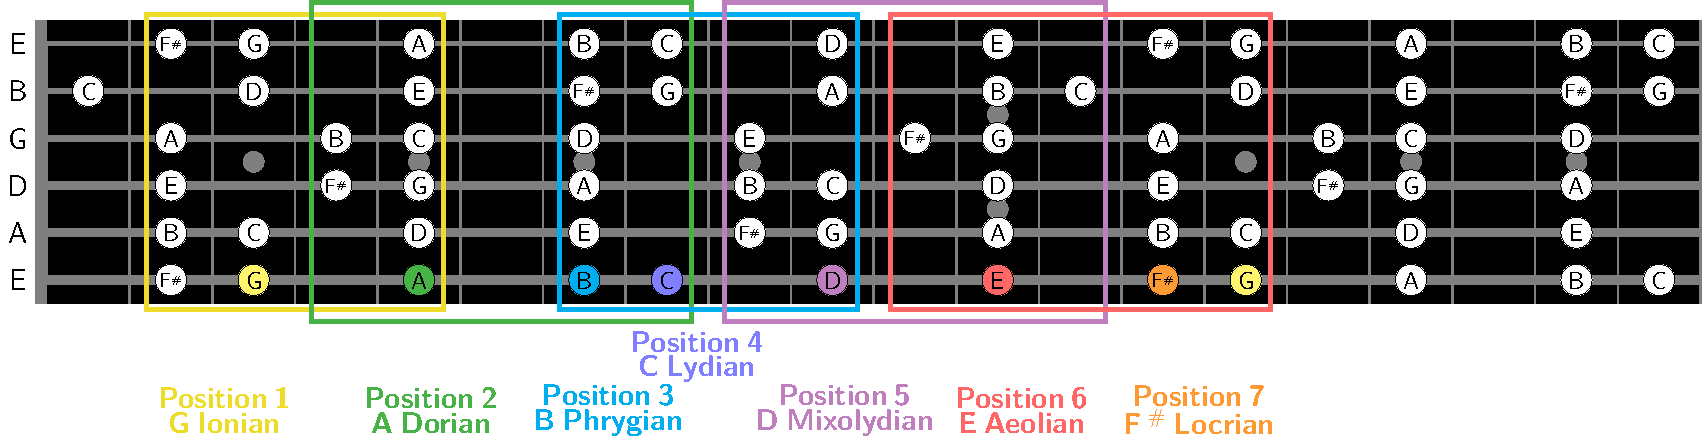
\includegraphics[scale=0.55, trim= {0cm 0cm 0cm 0cm}, clip]{Fretboard_MajorScale/main.pdf}
	\caption{G Major scale on the fretboard}
	\label{fig}
\end{figure}

% Figure 
\begin{figure}[h!]
	\centering
	\hspace*{-2cm}
	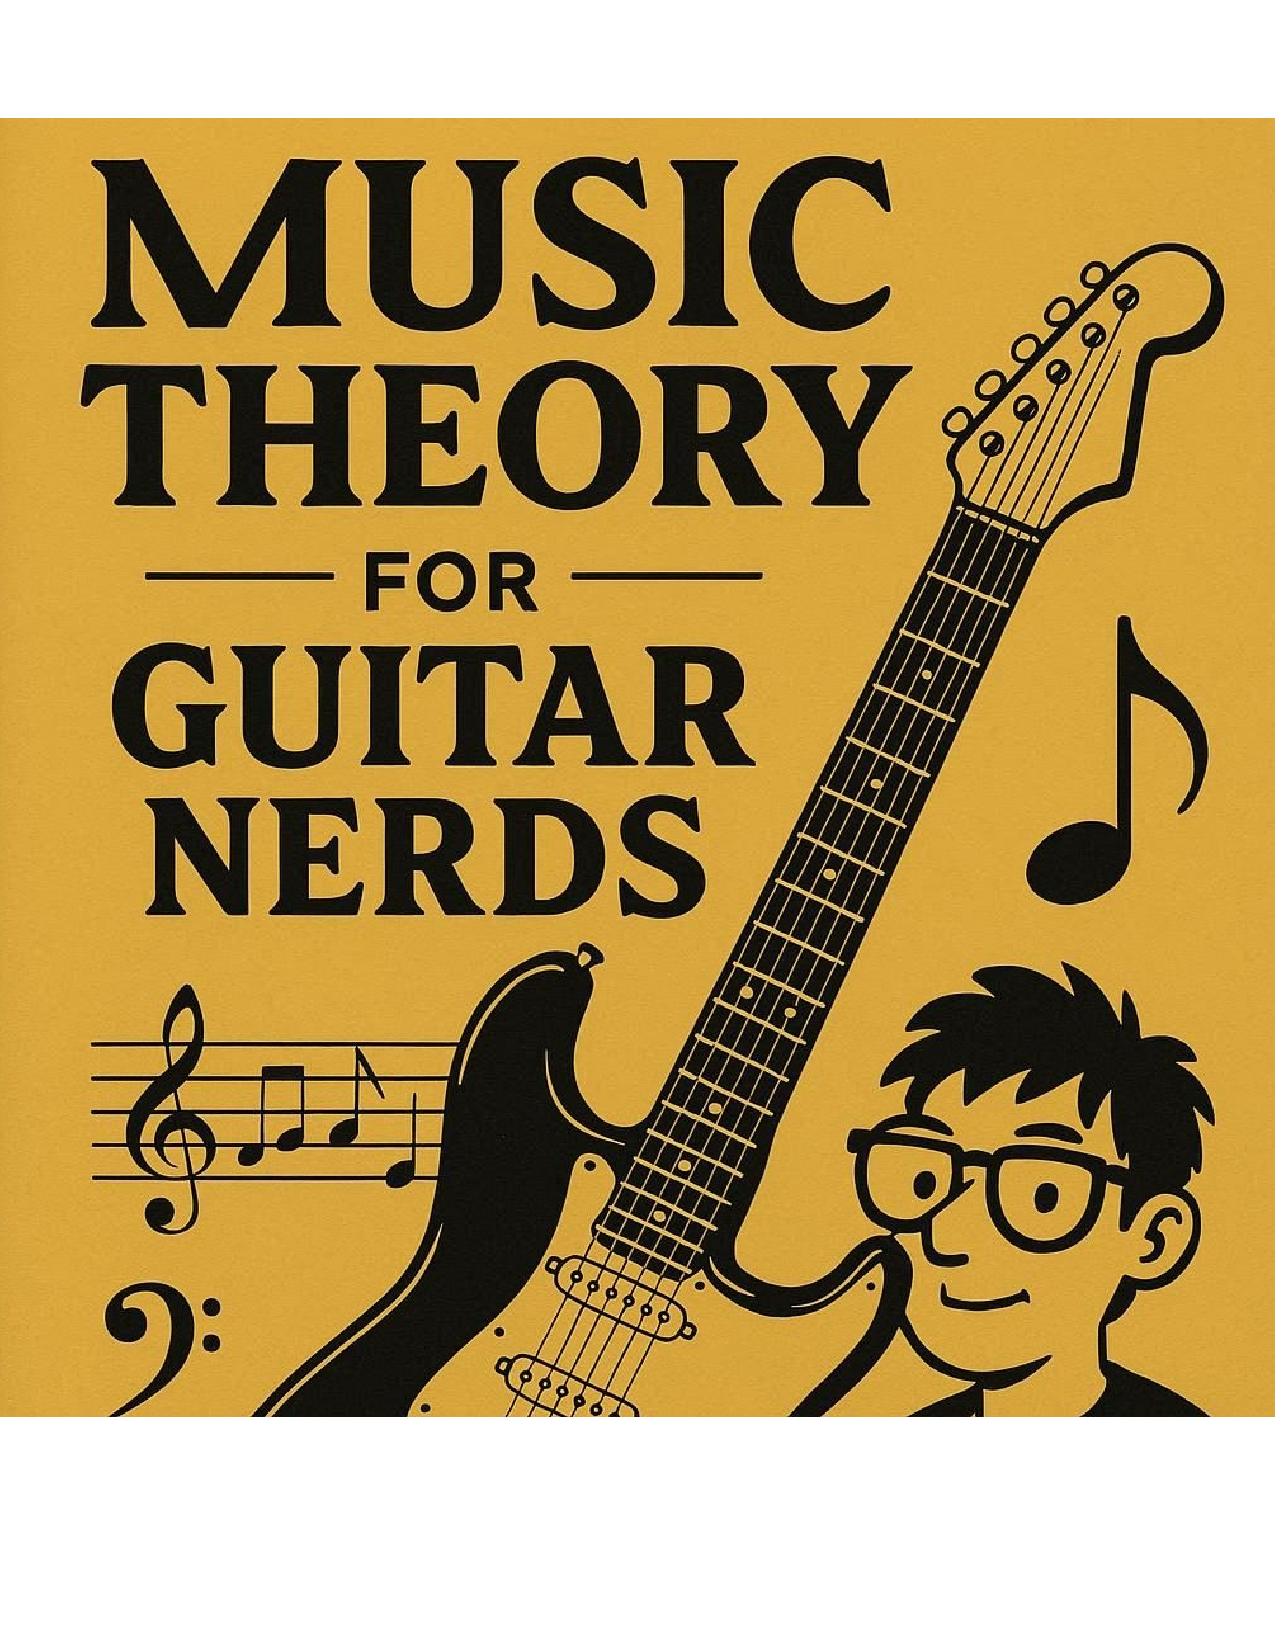
\includegraphics[scale=0.55, trim= {0cm 0cm 0cm 0cm}, clip]{Fretboard_pentatonic/main.pdf}
	\caption{Pattern of pentatonic scales}
	\label{fig}
\end{figure}

%%%%%%%%%%%%%%%%%%%%%%%%%%%%%%%%%%%%%%%%%%%%%%%%%%%%%%%%%%%%%%%%%%
% Construction of chords superimposing 3rds on a scale
\newpage
\section{Chords}

\begin{itemize}
	\item Tonic: I, iii, vi 
	\item Pre-dominant: IV, ii
	\item Dominant: V, vii$^\circ$
\end{itemize}


\begin{itemize}
	\item ``Sus'' chords: chord without third
	\item ``sus9'' will often replace the dominant 7th chord
\end{itemize}

%%%%%%%%%%%%%%%%%%%%%%%%%%%%%%%%%%%%%%%%%%%%%%%%%%%%%%%%%%%%%%%%%%%%%%%%%%%%%%%%%%%%%%%%%%%%%%%%%%%%%%%%%
\newpage
\subsection{Formation of chords}
% Table
% Source: 1997 - Vaillot Méthode Jazz
\begin{table*}[!h]
	\centering
	\caption{Construction of chords (notation is relative to the major scale)}
	\begin{tabular}{clcccccc}
		\hline \vspace{-0.2cm} \\
		$\#$ notes & Chords & & & & & &\\
		\hline \vspace{-0.2cm} \\ 
		\multirow{6}{*}{triad} & -        & 1 & M3 & 5 &  -  & -  & -\\
		                       & m        & 1 & m3 & 5 &  -  & -  & -\\
		                       & dim or $^\circ$  & 1 & m3 & b5  &  -  & -  & -\\
		                       & aug or $^\#$5 & 1 & m3 & $^\#$5 &  -  & -  & -\\
		                       & sus2     & 1 & M2  & 5     &  -  & -  & -\\
		                       & sus4     & 1 & 4   & 5     &  -  & -  & -\\
		\hline  
		\multirow{13}{*}{tetrad}& 7        & 1 & M3  & 5 & m7  & -  & -\\
		                       & $\Delta$  & 1 & M3  & 5 & M7  & -  & -\\
		                       & m$^7$     & 1 & m3  & 5 & m7  & -  & -\\
		                       & m$^\Delta$& 1 & m3  & 5 & M7  & -  & -\\
		                       & m$^{7\textrm{b}5}$ or $\varnothing$& 1 & m3  & b5 & m7  & -  & -\\
		                       & $^{\circ 7}$   & 1 & m3  & b5 & b7 & -  & -\\
                               & 6        & 1 & M3  & 5 & 6   & -  & -\\	
                               & m6       & 1 & m3  & 5 & 6   & -  & -\\	                       
		                       & m6(9)    & 1 & m3  & 6 & M9  & -  & -\\
		                       & 6(9)     & 1 & M3  & 6 & M9  & -  & -\\
		                       & 7sus4    & 1 & 4   & 5 & m7  & -  & -\\
		                       & add2     & 1 & M2  & M3& 5   & -  & -\\
		                       & add9     & 1 & M3  & 5 & M9  & -  & -\\
		\hline
		\multirow{6}{*}{pentad}& 7(b9)      & 1 & M3  & 5 & m7  & m9  & -\\
	                           & $\Delta^9$ & 1 & M3  & 5 & M7  & M9  & -\\
		                       & 9          & 1 & M3  & 5 & m7  & M9  & -\\
		                       & m9         & 1 & m3  & 5 & m7  & M9  & -\\
		                       & sus9       & 1 & 4   & 5 & m7  & M9  & -\\
		                       & 11         & 1 & 5   & m7& M9  & 11  & -\\ % The 3 is omitted to avoid the dissonace between 3-11.
		\hline
		\multirow{2}{*}{hexad} & 7(13)      & 1 & M3  & 5 & m7  & M9  & M13\\ % the 11 is omited to avoid the dissonance between 3-11.
		                       & 7(b9,13)   & 1 & M3  & 5 & m7  & m9  & M13\\
		\hline \vspace{-0.2cm}
	\end{tabular}
	\label{tab: }
\end{table*}

%%%%%%%%%%%%%%%%%%%%%%%%%%%%%%%%%%%%%%%%%%%%%%%%%%%%%%%%%%%%%%%%%%%%%%%%%%%%%%%%%%%%%%%%%%%%%%%%%%%%%%%%%
\newpage
\subsection{Chord inversions}

% Figure 
\begin{figure}[h!]
	\centering
	\hspace*{-2.2cm}
	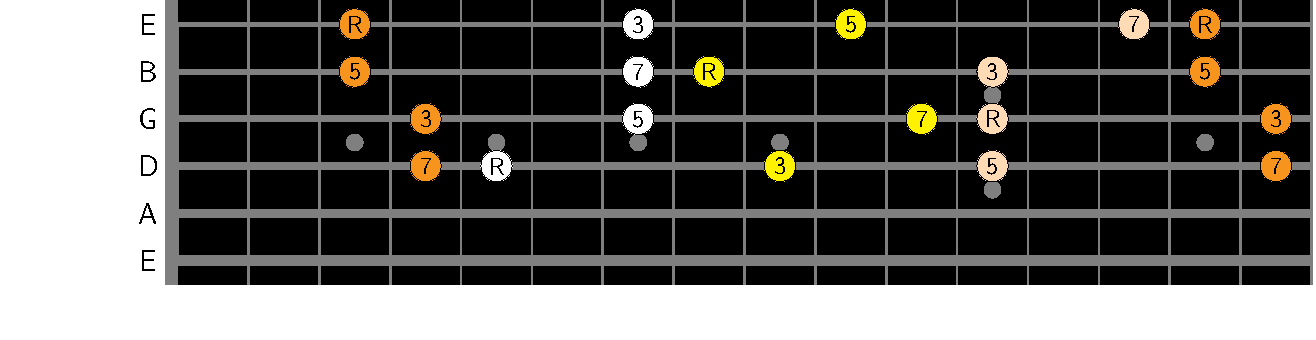
\includegraphics[scale=0.7, trim= {0cm 0cm 0cm 0cm}, clip]{figures/chord-inversions/maj7.pdf}
	\hspace*{-2.2cm}
	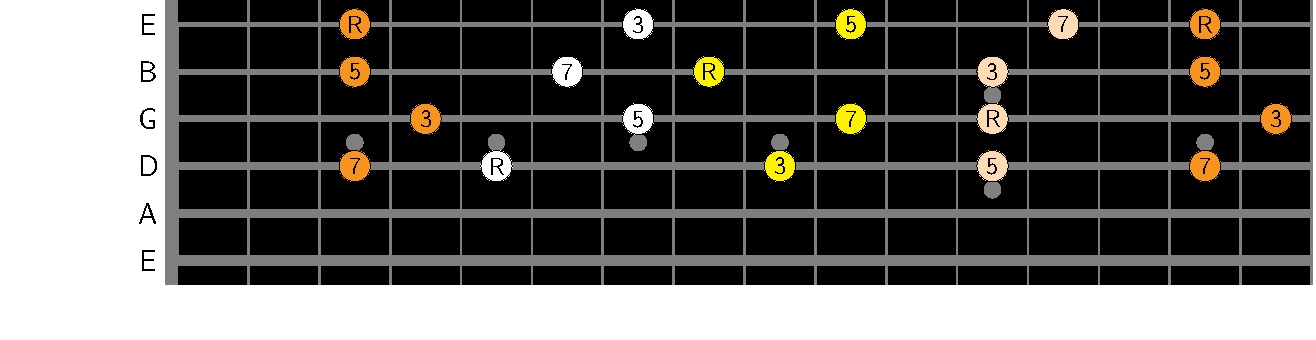
\includegraphics[scale=0.7, trim= {0cm 0cm 0cm 0cm}, clip]{figures/chord-inversions/Dominant7.pdf}
	\hspace*{-2.2cm}
	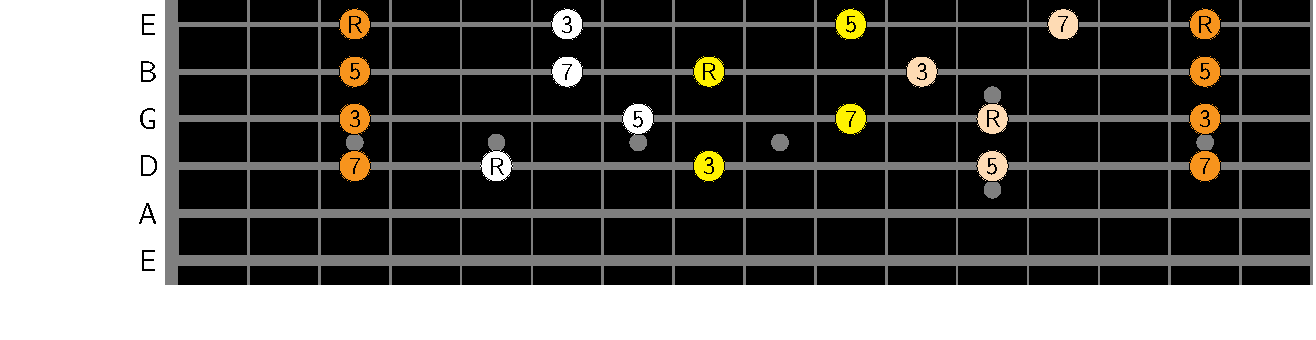
\includegraphics[scale=0.7, trim= {0cm 0cm 0cm 0cm}, clip]{figures/chord-inversions/m7.pdf}
	\caption{ }
	\label{fig}
\end{figure}



%%%%%%%%%%%%%%%%%%%%%%%%%%%%%%%%%%%%%%%%%%%%%%%%%%%%%%%%%%%%%%%%%%%%%%%%%%%%%%%%%%%%%%%%%%%%%%%%%%%%%%%%%
\newpage
\subsection{Chord progression and example}

% Table
% Source: 1997 - Vaillot Méthode Jazz
\begin{table*}[!h]
	\centering
	\caption{Famous chord progressions}
	\begin{adjustwidth}{-3cm}{}
	\begin{tabular}{p{5.0cm}p{5.5cm}p{7cm}}
		\hline \vspace{-0.2cm} \\
	    Name & Progression & Example\\
		\hline \vspace{-0.2cm} \\ 
		Pop major (punk)      & $\textrm{I}-\textrm{V}-\textrm{vi}-\textrm{IV}$ & Dammit, Let it be, Country Road \\
		Anatol (turnaround)   & $\textrm{I}^{\Delta}-\textrm{vi}^7-\textrm{ii}^7-\textrm{V}^7$ & Blue Moon \\
		50s progression       & $\textrm{I}-\textrm{vi}-\textrm{IV}-\textrm{V}$ & Every Breath You Take, Crocodile Rock\\
		Ragtime               &$\textrm{I}-\textrm{VI}^7-\textrm{II}^{7}-\textrm{V}^{7}$ & I want to be like you (Disney) \\
		Jazz (ii-V-I)         & $\textrm{ii}^{7}-\textrm{V}^7-\textrm{I}^{\Delta}$ & Autumn leaves\\
		Blues/Rock (Major)    & $\textrm{I}^7-\textrm{IV}^7-\textrm{V}^7-\textrm{I}^7$ & Johnny B. Goode\\
		
	    Mixo vamp (mixo)      & $\textrm{I}-\textrm{bVII}-\textrm{IV}-\textrm{I}$ & Hey Jude, Sweet home Alabama \\
	    Japanese ``Royal road'' & $\textrm{IV}^\Delta-\textrm{V}^7-\textrm{iii}^7-\textrm{vi}^7-$ {\footnotesize $(\textrm{ii}^7-\textrm{V}^7-\textrm{I}^{\Delta})$} & Shogo theme, anime \\
	    ``Storyteller''       & $\textrm{I}-\textrm{IV}-\textrm{vi}-\textrm{V}$ & \\
	    Creep chord            & I$\,-\,$III$\,-\,$IV$\,-\,$iv &  Creep, Space Oddity \\
		Pop minor             & $\textrm{i}-\textrm{bVI}-\textrm{bIII}-\textrm{bVII}$ & Save Tonight, Africa Toto \\	    
	    Aeolian vamp          & $\textrm{i}-\textrm{bVII}-\textrm{bVI}-\textrm{bVII}$  & Stairway to Heaven, All Iron Maiden \vspace{-0.8cm}  \\ 
		Minor progression 01    & $\textrm{i}-\textrm{i}-\textrm{bVI}-\textrm{V}$ & Sweet Dreams \\	    
	    Minor progression 02    & $\textrm{i}-\textrm{bVI}-\textrm{bIII}-\textrm{bVII}$ &  \\
	    Minor progression 03    & $\textrm{i}-\textrm{bVI}-\textrm{iv}-\textrm{bVII}$ & Final countdown\\
	    Minor progression 04    & $\textrm{i}-\textrm{bIII}-\textrm{bVII}-\textrm{iv}$ & Boulevard of Broken Dreams\\
	    Andalusian	(phrygian)& $\textrm{i}-\textrm{bVII}-\textrm{bVI}-\textrm{V}^7$ & Happy Together The Turtles\\
	    Blues/Rock (minor)      & $\textrm{i}^7-\textrm{iv}^7-\textrm{V}^7-\textrm{i}^7$ & Minor swing\\
	    Anime                   & $\textrm{bVI}-\textrm{bVII}-\textrm{i}$   &             \\ 
		Neapolitan              & i$\,-\,$bII$^6\,-\,$V$\,-\,$i &  Classic \\
		\hline \vspace{-0.2cm} \\
	\end{tabular}
	\end{adjustwidth}
	\label{tab:}
\end{table*}

Concepts: 
\begin{itemize}
	\item Borrowed chord: chord that is not built from the scale of the tonic. Examples:
	\begin{itemize}
		\item ``Picardy third'': a progression with an ending major triad instead of an expected minor triad to create an impression of resolution.
		\item Use the bVII
	\end{itemize}
	\item Transistion Chords:
	\begin{itemize}
		\item Secondary dominant chord (tonicization) (V/x): using the fifth of a chord (even if it's not a diatonic chord) in order to feel a ``resolution'' on this chord.
		\item Tritone substitution (Vsub/x or bV7/V): Approach any target chord with a diminished 7 chord a semitone above.
		\item Backdoor [ii V]. Approach the tonic with iv7 - bVII7 - I.
		\item Modulation (Rick Beato):
		\begin{itemize}
			\item Diatonic common chord (``close'' keys have many chords in common that can be used to modulate from a key to another. Common chords are called pivot chords)
			\item Chromatic pivot chord
			\item Enharmonic dominant
			\item Deceptive
			\item Enharmonic Dim7
			\item Dim7 to Dom7 (lower the root of the dim7 chord to create a dominant chord that leads to a new tonic)
			\item Chromatic Mediant
			\item Common tone (Pivot note)
			\item Direct or Linear (Abrupt change of key without preparation to ``lift'' the song)
			\item Chain Modulation ()
			\item Parallel modulation (Modulation of the mode but keep the same root ex: C to Cm)
		\end{itemize}
	\end{itemize}
\end{itemize}


% Figure 
\begin{figure}[h!]
	\centering
	\hspace*{-1cm}
	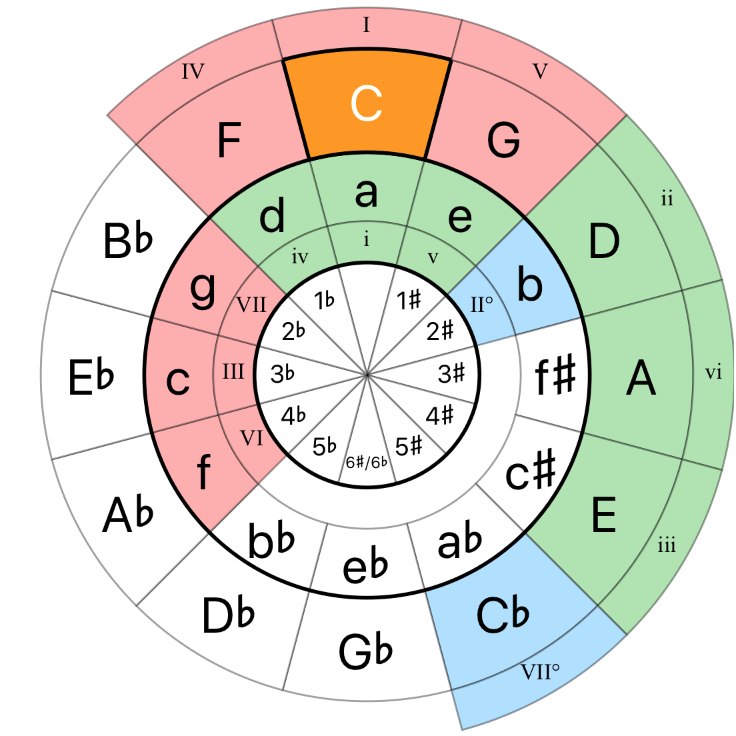
\includegraphics[scale=0.3, trim= {0cm 0cm 0cm 0cm}, clip]{Circle_5th.png}
	\caption{ }
	\label{fig}
\end{figure}

\begin{itemize}
	\item Substitution tritonique
	\item Substitution diatonique
\end{itemize}

%%%%%%%%%%%%%%%%%%%%%%%%%%%%%%%%%%%%%%%%%%%%%%%%%%%%%%%%%%%%%%%%%%
\newpage
\section{Modes}


% Table
\begin{table*}[!h]
	\caption{Table of modes }
	\begin{adjustwidth}{-2.3cm}{}
	\begin{tabular}{lccc cccc}
		\hline \vspace{-0.2cm} \\
		Major scale degree & I$^\Delta$ & ii$^{7}$ & iii$^{7}$ & IV$^\Delta$ & V$^7$ & vi$^{7}$ & vii$^{\varnothing}$ \\
		Mode & \textbf{Ionian} & \textbf{Dorian} & \textbf{Phrygian} & \textbf{Lydian} & \textbf{Mixolydian} & \textbf{Aeolian} & \textbf{Locrian}\\
		Example  & (joy) & (jazzy) & (flamenco) & (floaty, mystery) & (blues) & (sad) & (tension)\\		
		\hline \vspace{-0.2cm} \\ 
		{\scriptsize $\# \# \# \# \# \#$} & F$^\#$ & G$^\#$ & A$^\#$ & B & C$^\#$ & D$^\#$ & E$^\#$ \\
		{\scriptsize $\# \# \# \# \#$}    & B & C$^\#$ & D$^\#$ & E & F$^\#$ & G$^\#$ & A$^\#$\\
		{\scriptsize $\# \# \# \#$}       & E & F$^\#$ & G$^\#$ & A & B & C$^\#$ & D$^\#$\\
		{\scriptsize $\# \# \#$}          & A & B & C$^\#$ & D & E & F$^\#$ & G$^\#$\\
		{\scriptsize $\# \#$}             & D & E & F$^\#$ & G & A & B & C$^\#$\\
		{\scriptsize $\#$}                & G & A & B & C  & D & E & F$^\#$\\
		{\scriptsize -}                   & \textbf{C} & \textbf{D} & \textbf{E} & \textbf{F} & \textbf{G} & \textbf{A} & \textbf{B}\\
		{\scriptsize b}                   & F  & G  & A  & B$^\textrm{b}$ & C  & D  & E\\
		{\scriptsize bb}                  & B$^\textrm{b}$ & C     & D     & E$^\textrm{b}$ & F     & G     & A\\
		{\scriptsize bbb}                 & E$^\textrm{b}$ & F     & G     & A$^\textrm{b}$ & B$^\textrm{b}$ & C     & D\\
		{\scriptsize bbbb}                & A$^\textrm{b}$ & B$^\textrm{b}$ & C     & D$^\textrm{b}$ & E$^\textrm{b}$ & F     & G\\
		{\scriptsize bbbbb}               & D$^\textrm{b}$ & E$^\textrm{b}$ & F     & G$^\textrm{b}$ & A$^\textrm{b}$ & B$^\textrm{b}$ & C\\
		{\scriptsize bbbbbb}              & G$^\textrm{b}$ & A$^\textrm{b}$ & B$^\textrm{b}$ & C$^\textrm{b}$ & D$^\textrm{b}$ & E$^\textrm{b}$ & F\\
		\hline
		
		\hline \vspace{-0.2cm}
	\end{tabular}
	\label{tab: }
	\end{adjustwidth}
\end{table*}


% Table
\begin{table*}[!h]
	\caption{harmonization of scales}
	\begin{adjustwidth}{0cm}{}
	\begin{tabular}{r|ccc cccc}
		\hline \vspace{-0.4cm} \\
		\multirow{2}{*}{Major}          & 1 & 2 & 3 & 4 & 5 & 6 & 7\\ 
		                                & I$^\Delta$ & ii$^{7}$ & iii$^{7}$ & IV$^\Delta$ & V$^7$ & vi$^{7}$ & vii$^{\varnothing}$ \\
		\hline \vspace{-0.2cm} \\
		\multirow{2}{*}{Minor natural} & 1 & 2 & b3 & 4 & 5 & b6 & b7\\ 
		                                & i$^7$ & ii$^{\varnothing}$ & bIII$^{\Delta}$ & iv$^7$ & v$^7$ & bVI$^{\Delta}$ & bVII$^{7}$ \\
		\hline \vspace{-0.2cm} \\
		\multirow{2}{*}{Harmonic minor} & 1 & 2 & b3 & 4 & 5 & b6 & 7\\ 
		                                & i$^{\Delta}$ & ii$^{\varnothing}$ & bIII$^{\Delta, \textrm{aug}}$ & iv$^7$ & V$^7$ & bVI$^{\Delta}$ & vii$^{\circ 7}$ \\
		\hline \vspace{-0.2cm} \\
		\multirow{2}{*}{Melodic minor} & 1 & 2 & b3 & 4 & 5 & 6 & 7\\ 
			                           & i$^{\Delta}$ & ii$^{7}$ & bIII$^{\Delta, \textrm{aug}}$ & IV$^7$ & V$^7$ & vi$^{\varnothing}$ & vii$^{\varnothing}$ \\
			                           \hline \vspace{-0.2cm} \\
		\multirow{2}{*}{Dorian}        & 1 & 2 & b3 & 4 & 5 & 6 & b7\\ 
			                           & i$^{7}$ & ii$^{7}$ & bIII$^{\Delta}$ & IV$^7$ & v$^7$ & vi$^{\varnothing}$ & bVII$^{\Delta}$ \\
		\hline 
	\end{tabular}
	\label{tab: }
	\end{adjustwidth}
\end{table*}

\begin{itemize}
	\item Ionian (Joy), dorian(Jazz), phrygian(flamenco,doom), lydian (floaty,mystery) (ex: E.T., Jurassic Park, Back to the Future), mixo(blues)(ex: AC/DC), aeolian(sad)(ex: Losing my Religion), locrian(tension)(ex:Bjork Army of Me) 
	\item Harmonization of harmonic minor scale
	\item Harmonization of melodic minor scale
	\item How to use this table
	\item Example of chord progression
\end{itemize}


%%%%%%%%%%%%%%%%%%%%%%%%%%%%%%%%%%%%%%%%%%%%%%%%%%%%%%%%%%%%%%%%%%
\newpage
\section{Arpeggios}

% Figure
\begin{table}[!h]
	\hspace*{-4cm}
	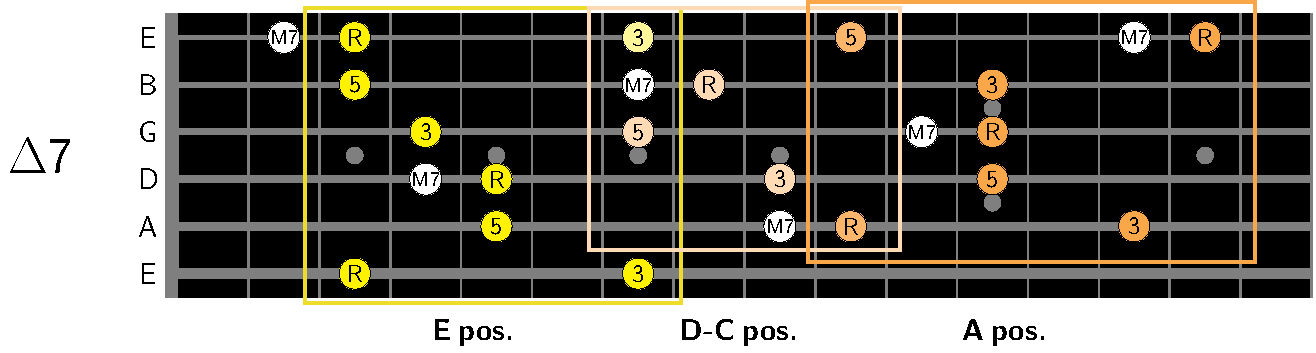
\includegraphics[width=10.5cm, trim= {0cm 0cm 0cm 0cm}, clip]{Arpeges/maj7_chords.pdf}
	\hspace*{-1cm}
	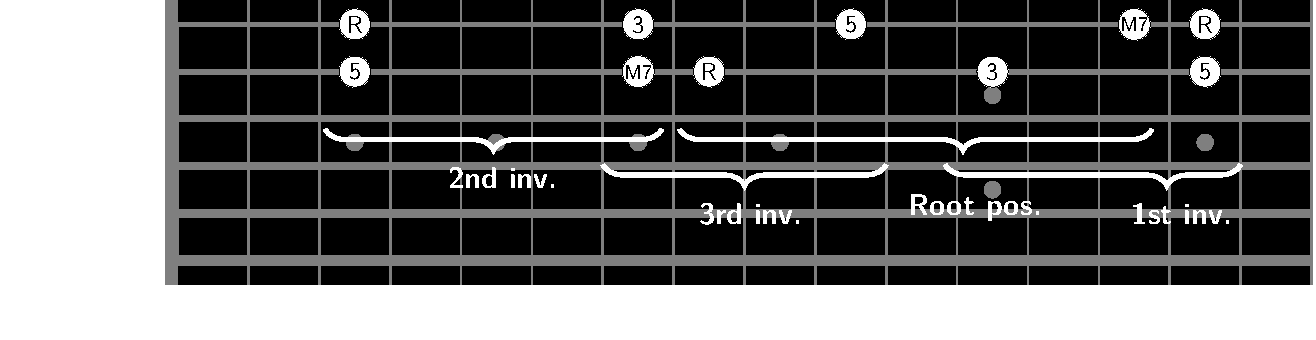
\includegraphics[width=10.5cm, trim= {0cm 0cm 0cm 0cm}, clip]{Arpeges/2notes_maj7_chords.pdf}
	
	\hspace*{-4cm}
	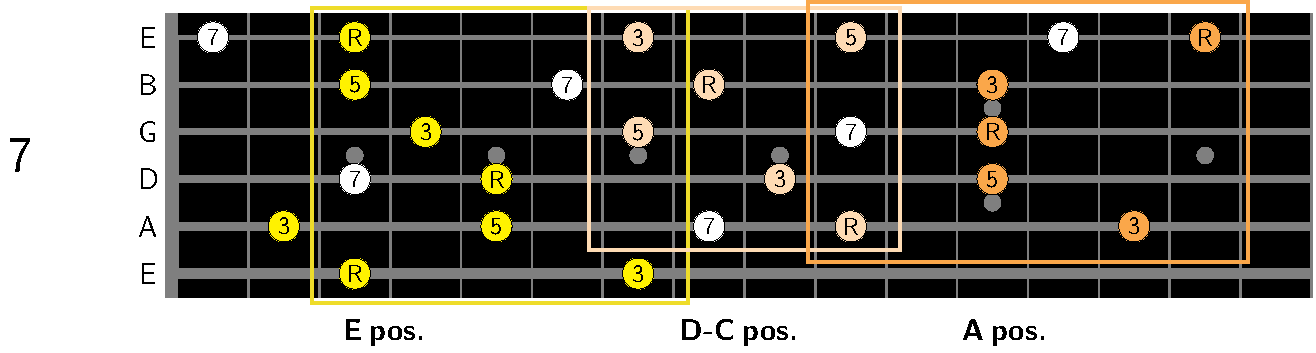
\includegraphics[width=10.5cm, trim= {0cm 0cm 0cm 0cm}, clip]{Arpeges/dom7_chords.pdf}
	\hspace*{-1cm}
	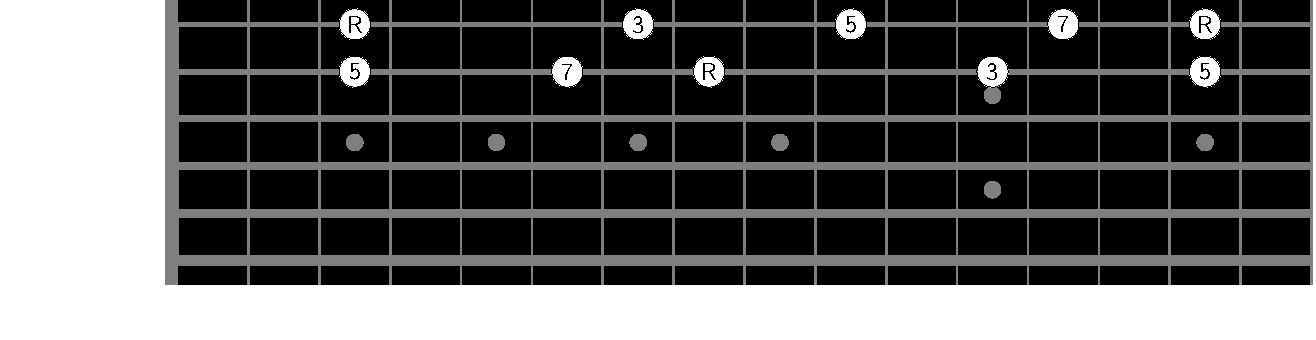
\includegraphics[width=10.5cm, trim= {0cm 0cm 0cm 0cm}, clip]{Arpeges/2notes_dom7_chords.pdf}
	
	\hspace*{-4cm}
	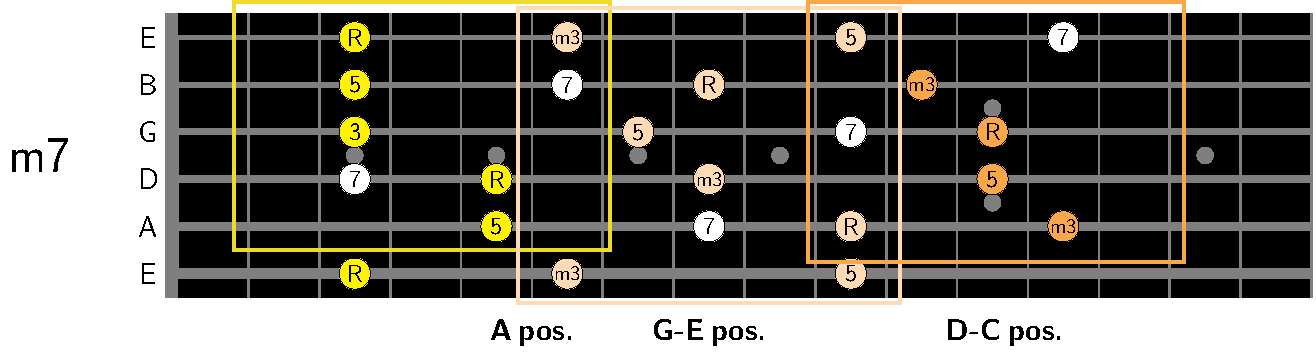
\includegraphics[width=10.5cm, trim= {0cm 0cm 0cm 0cm}, clip]{Arpeges/m7_chords.pdf}
	\hspace*{-1cm}
	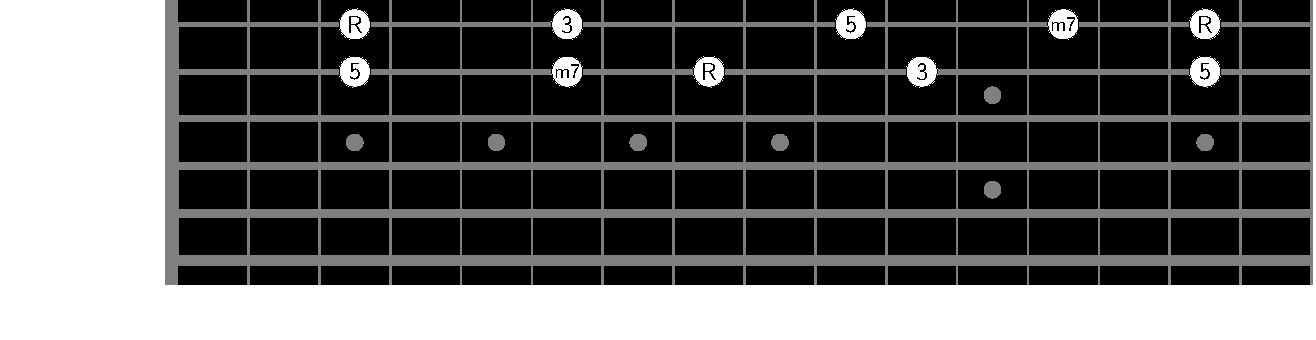
\includegraphics[width=10.5cm, trim= {0cm 0cm 0cm 0cm}, clip]{Arpeges/2notes_m7_chords.pdf}
	
	\hspace*{-4cm}
	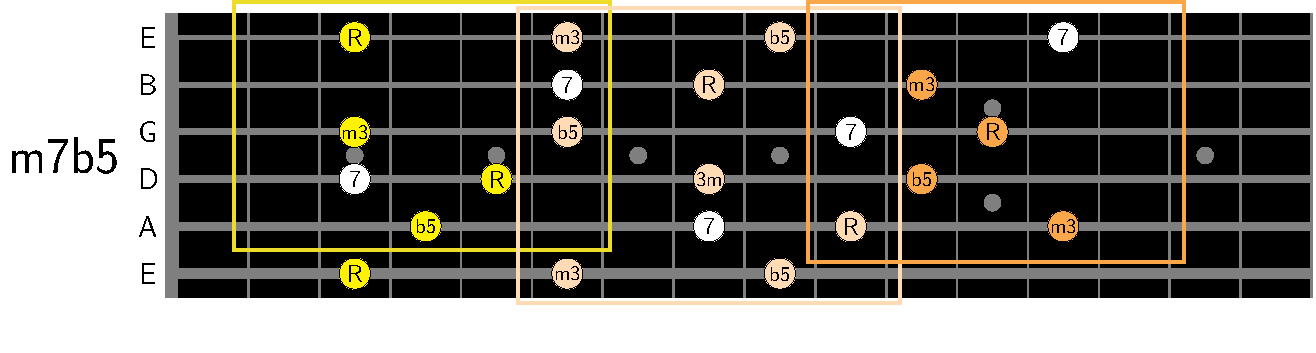
\includegraphics[width=10.5cm, trim= {0cm 0cm 0cm 0cm}, clip]{Arpeges/m7b5_chords.pdf}
	\hspace*{-1cm}
	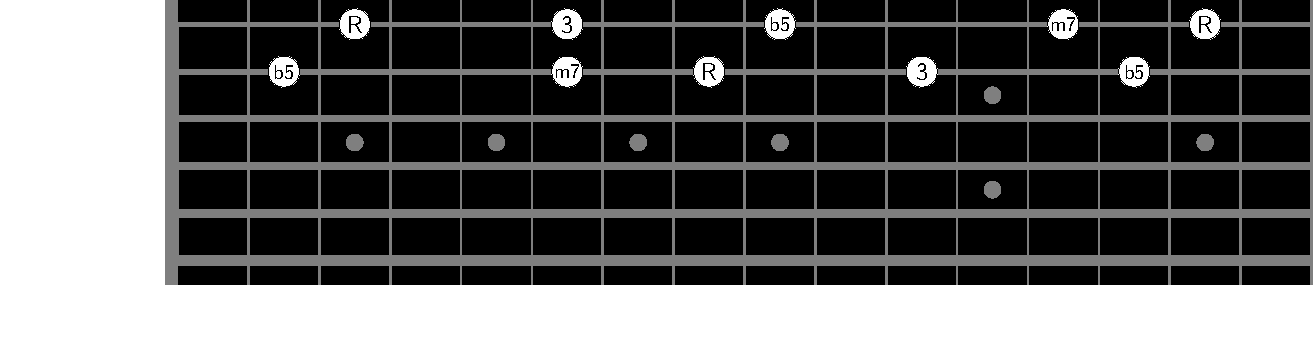
\includegraphics[width=10.5cm, trim= {0cm 0cm 0cm 0cm}, clip]{Arpeges/2notes_m7b5_chords.pdf}
	\caption{G arpeggio}
	\label{fig}
\end{table}


%%%%%%%%%%%%%%%%%%%%%%%%%%%%%%%%%%%%%%%%%%%%%%%%%%%%%%%%%%%%%%%%%%
\newpage
\section{Transposition}

https://www.youtube.com/watch?v=Vxac3hHrxg8


%%%%%%%%%%%%%%%%%%%%%%%%%%%%%%%%%%%%%%%%%%%%%%%%%%%%%%%%%%%%%%%%%%
\newpage
\section{Blues}

% Table
\begin{table*}[!h]
	\caption{Blues scales (relative to the major scale)}
	\centering
	%\begin{adjustwidth}{0cm}{}
	\begin{tabular}{l|cccccccc}
		Scale name  & \multicolumn{8}{c}{Formula} \\ 
		\hline \hline \vspace{-0.4cm} \\
		Blues Major   & 1 & 2  & \textcolor{red}{b3} & 3  &   -   & 5  & 6  &  -  \\ 
		Blues minor   & 1 &  - & b3 & 4  & \textcolor{red}{b5} &  5  & - &  b7 \\ 
	\end{tabular}
	\label{tab: }
	%\end{adjustwidth}
\end{table*}

% Table
\begin{table*}[!h]
	\caption{12 bar blues in C major}
	\centering
	\begin{tabular}{| c | c | c | c |}
		\hline
		\phantom{x}C7\phantom{x} & \phantom{x}C7\phantom{x} & \phantom{x}C7\phantom{x} & \phantom{x}C7\phantom{x}  \\ 
		\hline
		\phantom{x}F7\phantom{x} & \phantom{x}F7\phantom{x} & \phantom{x}C7\phantom{x} & \phantom{x}C7\phantom{x}  \\ 
		\hline
		\phantom{x}G7\phantom{x} & \phantom{x}F7\phantom{x} & \phantom{x}C7\phantom{x} & \phantom{x}G7\phantom{x}  \\ 
		\hline
	\end{tabular}
	\label{tab: }
\end{table*}

% Figure 
\begin{figure}[h!]
	\centering
	\hspace*{-1cm}
	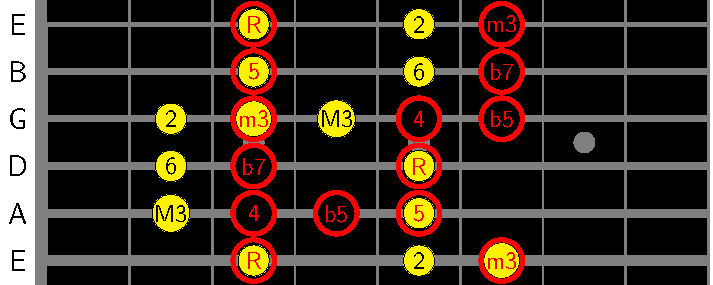
\includegraphics[width=8cm, trim= {0cm 0cm 0cm 0cm}, clip]{Blues/main.pdf}
	\caption{ }
	\label{fig}
\end{figure}

%%%%%%%%%%%%%%%%%%%%%%%%%%%%%%%%%%%%%%%%%%%%%%%%%%%%%%%%%%%%%%%%%%
\newpage
\section{Composition variation (Shred Master Scott)}

\begin{itemize}
	\item Pedal tone
	\item Inversion
	\item Voice leading
\end{itemize}

\newpage
\bibliographystyle{plain}
\bibliography{/home/jh/Documents/library.bib}

\end{document}
